% mnras_template.tex 
%
% LaTeX template for creating an MNRAS paper
%
% v3.0 released 14 May 2015
% (version numbers match those of mnras.cls)
%
% Copyright (C) Royal Astronomical Society 2015
% Authors:
% Keith T. Smith (Royal Astronomical Society)

% Change log
%
% v3.2 July 2023
%	Updated guidance on use of amssymb package
% v3.0 May 2015
%    Renamed to match the new package name
%    Version number matches mnras.cls
%    A few minor tweaks to wording
% v1.0 September 2013
%    Beta testing only - never publicly released
%    First version: a simple (ish) template for creating an MNRAS paper

%%%%%%%%%%%%%%%%%%%%%%%%%%%%%%%%%%%%%%%%%%%%%%%%%%
% Basic setup. Most papers should leave these options alone.
\documentclass[fleqn,usenatbib,openbib]{mnras}

% MNRAS is set in Times font. If you don't have this installed (most LaTeX
% installations will be fine) or prefer the old Computer Modern fonts, comment
% out the following line
\usepackage{newtxtext,newtxmath}
% Depending on your LaTeX fonts installation, you might get better results with one of these:
%\usepackage{mathptmx}
%\usepackage{txfonts}

% Use vector fonts, so it zooms properly in on-screen viewing software
% Don't change these lines unless you know what you are doing
\usepackage[T1]{fontenc}

% Allow "Thomas van Noord" and "Simon de Laguarde" and alike to be sorted by "N" and "L" etc. in the bibliography.
% Write the name in the bibliography as "\VAN{Noord}{Van}{van} Noord, Thomas"
\DeclareRobustCommand{\VAN}[3]{#2}
\let\VANthebibliography\thebibliography
\def\thebibliography{\DeclareRobustCommand{\VAN}[3]{##3}\VANthebibliography}


%%%%% AUTHORS - PLACE YOUR OWN PACKAGES HERE %%%%%

\usepackage[spanish]{babel}
\usepackage{lipsum}
\usepackage{url}
\usepackage{pgfplots}
\usepackage{booktabs, colortbl, bigstrut}

% Only include extra packages if you really need them. Avoid using amssymb if newtxmath is enabled, as these packages can cause conflicts. newtxmatch covers the same math symbols while producing a consistent Times New Roman font. Common packages are:
\usepackage{graphicx}	% Including figure files
\usepackage{amsmath}	% Advanced maths commands

%%%%%%%%%%%%%%%%%%%%%%%%%%%%%%%%%%%%%%%%%%%%%%%%%%

%%%%% AUTHORS - PLACE YOUR OWN COMMANDS HERE %%%%%

\usepackage[nameinlink,noabbrev]{cleveref}
\crefformat{figure}{\textsuperscript{#2#1#3}}
\crefformat{table}{\textsuperscript{#2#1#3}}

\addto\captionsspanish{\renewcommand{\refname}{REFERENCIAS}}

\makeatletter
\def\@abstract{\list{}{%
    \listparindent\realparindent
    \itemindent\z@
    \labelwidth\z@ \labelsep\z@
    \leftmargin\z@\rightmargin\z@%%was 11pc left
    \parsep 0pt plus 1pt}\item[]%
    \reset@font\normalsize{\bf PRESENTACIÓN}\\\reset@font\abslarge
} % SFB 0.1.01
\def\@keywords{\list{}{%
    \labelwidth\z@ \labelsep\z@
    \leftmargin\z@\rightmargin\z@  %was 11pc left was 11pc\right....
    \parsep 0pt plus 1pt}\item[]\reset@font\abslarge{\bf Palabras clave: }%
}
\makeatother

\renewcommand\theequation{\Alph{equation}}

% Please keep new commands to a minimum, and use \newcommand not \def to avoid
% overwriting existing commands. Example:
%\newcommand{\pcm}{\,cm$^{-2}$}	% per cm-squared

%%%%%%%%%%%%%%%%%%%%%%%%%%%%%%%%%%%%%%%%%%%%%%%%%%

%%%%%%%%%%%%%%%%%%% TITLE PAGE %%%%%%%%%%%%%%%%%%%

% Title of the paper, and the short title which is used in the headers.
% Keep the title short and informative.
\title[Ondas Estacionarias]{Determinación de la densidad lineal de un hilo mediante la observación del mismo oscilando en resonancia}

% The list of authors, and the short list which is used in the headers.
% If you need two or more lines of authors, add an extra line using \newauthor
\author[Álvaro Jerónimo Sánchez]{
Álvaro Jerónimo Sánchez$^{1}$, DNI: 09847051S.\thanks{E-mail: alvaro.jeronimos@estudiante.uam.es}
Copartícipe: Hugo Pérez Hernández$^{1}$
\\
% List of institutions
$^{1}$Universidad Autónoma de Madrid, Ciudad universitaria de Cantoblanco, 28049,España \\
Facultad de Ciencias, Grado en Química, FÍSICA I
}

% These dates will be filled out by the publisher
\date{Prácticas 14/09/2023. Informe 17/10/2023. Fecha Límite 23/10/2023}

% Enter the current year, for the copyright statements etc.
\pubyear{2023}

% Don't change these lines
\begin{document}
\label{firstpage}
\pagerange{\pageref{firstpage}--\pageref{lastpage}}
\maketitle

%%%%%%%%%%%%%%%%%%%%%%%%%%%%%%%%%%%%%%%%%%%%%%%%%%

%%%%%%%%%%%%%%%%% BODY OF PAPER %%%%%%%%%%%%%%%%%%
\begin{abstract}

El estudio de una onda nos permite deducir diversas características de la misma a través de pocos datos recogidos, debido a que esta tiene características predecibles. Esta práctica tiene como objetivo hallar la densidad lineal de un hilo oscilante estudiando sus propiedades (en este caso: frecuencia, longitud, modo de oscilación y tensión) cuando la onda que traza (unidimensional, forzada y cerrada) se encuentra en resonancia, generando ondas estacionarias.
\vspace{1cm}
\end{abstract}

%%%%%%%%%%%%%%%%%%%%%%%%%%%%%%%%%%%%%%%%%%%%%%%%%%
\section{Teoría}

Las ondas son perturbaciones que transportan energía por el espacio. Es un cambio de estado de un sistema de manera periódica en el espacio y el tiempo (\cite{2002Hop}) Estas perturbaciones pueden ser visibles o no (e.g. una onda sonora, que se trata de oscilaciones de partículas en el aire) y, a excepción de las ondas elecromagnéticas, requieren un medio para generarse. La onda que se ha observado en esta práctica se trata de una onda mecánica transversal (la perturbación es paralela a la propagación de la onda) y unidimensional formada en un hilo de goma elástica mediante un oscilador. Esta se trata de una onda forzada de sistema cerrado, ya que la oscilación es causa de una fuerza externa aplicada y los dos extremos están cerrados, lo que dará lugar a un ''rebote'' de la perturbación; y, al no estar presente la fricción, se trata de una onda sin amortiguar.

Debido a que es un sistema de oscilaciones forzadas y la fuerza externa es periódica, si el oscilador vibra a la frecuencia de la fuerza externa, llegará al estado de \textbf{resonancia} (\cite{2002Hop}). Este hecho se puede observar fácilmente, ya que se podrá apreciar claramente la forma de la onda con sus nodos y vientres, estando los máximos de los vientres aparentemente quietos, y los nodos con cierta vibración.

 Una onda está formada por varias \underline{\smash{componentes}}\cref{fig:componentes} resultantes de la oscilación:
 
 \begin{figure}
    \centering
    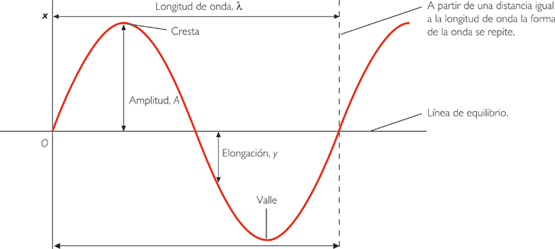
\includegraphics[width=\columnwidth]{componentes.png}
    \caption{Las componentes de una onda unidimensional \protect\cite{onda}}
    \label{fig:componentes}
    \end{figure}
 \begin{itemize}

\item \textbf{Elongación ($x$):} Diferencia de la distancia de un punto al equilibrio.
\item \textbf{Amplitud ($A$):} Elongación máxima de una onda en valor absoluto. 
\item \textbf{Nodo:} Punto de una onda con mayor velocidad de oscilación ($v_o$).
\item \textbf{Vientre:} Espacio entre nodo y nodo.
\item \textbf{Longitud de onda ($\lambda$):} Distancia entre dos nodos de una onda.
\item \textbf{Frecuencia ($\nu$):} Número de oscilaciones que ocurren en un tiempo determinado. Su inversa es el \textbf{periodo}.
\item \textbf{Fase($\phi$):} Define el estado oscilatorio de la onda. Ángulo que hay entre el equilibrio y un punto de una onda en un instante (en radianes).

 \end{itemize}

%%%%%%%%%%%%%%%%%%%%%%%%%%%%%%%%%%%%%%%%%%%%%%%%%%
\section{Montaje experimental}

\subsection{Instrumentos}

Para esta práctica se ha situado un vibrador electromecánico a $L\approxeq 1.6$ m (medido con una regla milimetrada de $1$ m) y se ha ajustado la tensión de un hilo de goma elástica a $0.4$ N empleando un dinamómetro con un error de $\pm 0.01$ N. A continuación se ha encendido el generador de funciones (U21015 VENTUS), y se ha configurado en el modo de onda sinusoidal (\cite{osc}). Dicho generador está alimentado por $12$ V AC (\cite{labuam}), y éste suministra una corriente periódica al vibrador (que causa las subidas y bajadas del enganche), creando el movimiento oscilatorio. El oscilador puede suministrar hasta $1$ A, y permite variar la amplitud (sin medida alguna, de manera porcentual), el tipo de onda y la frecuencia. 

\subsection{Medición}

Una vez situado el vibrador a $L\approxeq 1.6$ m con una tensión en la cuerda de $0.4$ N y con el modo de onda sinusoidal, se ha cambiado la unidad de medida del oscilador a \textit{Hz} (inicialmente se encuentra en \textit{kHz}) y se ha establecido la frecuencia en $40$ Hz, con una amplitud del $25\%$, suficiente en un principio para poder observar la forma de la onda.

A continuación se fue ajustando la frecuencia (de manera decreciente) poco a poco hasta lograr la resonancia. La primera de las veces en las que se llegó a este estado se observaron 10 vientres (el número de ondas $k=10$). Se anotó en una tabla la frecuencia con la que estaba oscilando la onda en esa resonacia, y se reanudó el decrecimiento de la frecuencia hasta llegar a la siguiente resonancia. Se repitió la toma de datos de frecuencia para cada resonancia, cada vez perdiendo una unidad del número de ondas, hasta llegar a $k=1$ (el modo fundamental de la onda). Para las frecuencias más bajas se necesitó incrementar ligeramente la amplitud, ya que con ésta al $25\%$ resultaba más difícil discernir la forma de la onda.

Este mismo proceso y las tomas de medidas se repitieron de forma idéntica ajustando la tensión a $0.7$ N y $1.0$ N. Como era de esperar, cuanto mayor el valor de la tensión, mayor la frecuencia correspondiente a cada estado de resonancia.

% Table generated by Excel2LaTeX from sheet 'Sheet2'
\begin{table}
    \scriptsize
    \centering
    \caption{Frecuencias correspondientes a cada resonancia con distintas tensiones y la densidad lineal calculada con dichos valores}
      \begin{tabular}{|rr|r|r|r|r|r|r|}
      \hline
      \rowcolor[rgb]{ .788,  .788,  .788} \multicolumn{2}{|r|}{\small{Tensión}} & \multicolumn{2}{c|}{\small{0.4 N}} & \multicolumn{2}{c|}{\small{0.7 N}} & \multicolumn{2}{c|}{\small{1 N}} \bigstrut\\
  \cline{2-8}    \rowcolor[rgb]{ .788,  .788,  .788} \multicolumn{1}{|c|}{} & \multicolumn{1}{c|}{\cellcolor[rgb]{ .929,  .929,  .929}k} & \multicolumn{1}{c|}{\cellcolor[rgb]{ .929,  .929,  .929}$\nu$ (Hz)} & \multicolumn{1}{c|}{\cellcolor[rgb]{ .929,  .929,  .929}$\rho$ (kg/m)} & \multicolumn{1}{c|}{\cellcolor[rgb]{ .929,  .929,  .929}$\nu$ (Hz)} & \multicolumn{1}{c|}{\cellcolor[rgb]{ .929,  .929,  .929}$\rho$ (kg/m)} & \multicolumn{1}{c|}{\cellcolor[rgb]{ .929,  .929,  .929}$\nu$ (Hz)} & \multicolumn{1}{c|}{\cellcolor[rgb]{ .929,  .929,  .929}$\rho$ (kg/m)} \bigstrut\\
  \cline{2-8}    \rowcolor[rgb]{ .788,  .788,  .788} \multicolumn{1}{|c|}{} & \multicolumn{1}{c|}{\cellcolor[rgb]{ 1,  1,  1}10} & \multicolumn{1}{c|}{\cellcolor[rgb]{ 1,  1,  1}37.60} & \cellcolor[rgb]{ 1,  1,  1}2.7630E-03 & \multicolumn{1}{c|}{\cellcolor[rgb]{ 1,  1,  1}48.60} & \cellcolor[rgb]{ 1,  1,  1}2.8942E-03 & \multicolumn{1}{c|}{\cellcolor[rgb]{ 1,  1,  1}57.80} & \cellcolor[rgb]{ 1,  1,  1}2.9231E-03 \bigstrut\\
  \cline{2-8}    \rowcolor[rgb]{ .788,  .788,  .788} \multicolumn{1}{|c|}{} & \multicolumn{1}{c|}{\cellcolor[rgb]{ 1,  1,  1}9} & \multicolumn{1}{c|}{\cellcolor[rgb]{ 1,  1,  1}34.60} & \cellcolor[rgb]{ 1,  1,  1}2.6430E-03 & \multicolumn{1}{c|}{\cellcolor[rgb]{ 1,  1,  1}43.40} & \cellcolor[rgb]{ 1,  1,  1}2.9397E-03 & \multicolumn{1}{c|}{\cellcolor[rgb]{ 1,  1,  1}51.50} & \cellcolor[rgb]{ 1,  1,  1}2.9824E-03 \bigstrut\\
  \cline{2-8}    \rowcolor[rgb]{ .788,  .788,  .788} \multicolumn{1}{|c|}{} & \multicolumn{1}{c|}{\cellcolor[rgb]{ 1,  1,  1}8} & \multicolumn{1}{c|}{\cellcolor[rgb]{ 1,  1,  1}30.60} & \cellcolor[rgb]{ 1,  1,  1}2.6699E-03 & \multicolumn{1}{c|}{\cellcolor[rgb]{ 1,  1,  1}38.70} & \cellcolor[rgb]{ 1,  1,  1}2.9212E-03 & \multicolumn{1}{c|}{\cellcolor[rgb]{ 1,  1,  1}45.90} & \cellcolor[rgb]{ 1,  1,  1}2.9666E-03 \bigstrut\\
  \cline{2-8}    \rowcolor[rgb]{ .788,  .788,  .788} \multicolumn{1}{|c|}{} & \multicolumn{1}{c|}{\cellcolor[rgb]{ 1,  1,  1}7} & \multicolumn{1}{c|}{\cellcolor[rgb]{ 1,  1,  1}26.60} & \cellcolor[rgb]{ 1,  1,  1}2.7052E-03 & \multicolumn{1}{c|}{\cellcolor[rgb]{ 1,  1,  1}33.80} & \cellcolor[rgb]{ 1,  1,  1}2.9320E-03 & \multicolumn{1}{c|}{\cellcolor[rgb]{ 1,  1,  1}39.90} & \cellcolor[rgb]{ 1,  1,  1}3.0057E-03 \bigstrut\\
  \cline{2-8}    \rowcolor[rgb]{ .788,  .788,  .788} \multicolumn{1}{|c|}{} & \multicolumn{1}{c|}{\cellcolor[rgb]{ 1,  1,  1}6} & \multicolumn{1}{c|}{\cellcolor[rgb]{ 1,  1,  1}23.00} & \cellcolor[rgb]{ 1,  1,  1}2.6583E-03 & \multicolumn{1}{c|}{\cellcolor[rgb]{ 1,  1,  1}28.70} & \cellcolor[rgb]{ 1,  1,  1}2.9877E-03 & \multicolumn{1}{c|}{\cellcolor[rgb]{ 1,  1,  1}34.00} & \cellcolor[rgb]{ 1,  1,  1}3.0412E-03 \bigstrut\\
  \cline{2-8}    \rowcolor[rgb]{ .788,  .788,  .788} \multicolumn{1}{|c|}{} & \multicolumn{1}{c|}{\cellcolor[rgb]{ 1,  1,  1}5} & \multicolumn{1}{c|}{\cellcolor[rgb]{ 1,  1,  1}19.00} & \cellcolor[rgb]{ 1,  1,  1}2.7052E-03 & \multicolumn{1}{c|}{\cellcolor[rgb]{ 1,  1,  1}24.40} & \cellcolor[rgb]{ 1,  1,  1}2.8705E-03 & \multicolumn{1}{c|}{\cellcolor[rgb]{ 1,  1,  1}28.40} & \cellcolor[rgb]{ 1,  1,  1}3.0269E-03 \bigstrut\\
  \cline{2-8}    \rowcolor[rgb]{ .788,  .788,  .788} \multicolumn{1}{|c|}{} & \multicolumn{1}{c|}{\cellcolor[rgb]{ 1,  1,  1}4} & \multicolumn{1}{c|}{\cellcolor[rgb]{ 1,  1,  1}15.10} & \cellcolor[rgb]{ 1,  1,  1}2.7411E-03 & \multicolumn{1}{c|}{\cellcolor[rgb]{ 1,  1,  1}19.30} & \cellcolor[rgb]{ 1,  1,  1}2.9363E-03 & \multicolumn{1}{c|}{\cellcolor[rgb]{ 1,  1,  1}22.70} & \cellcolor[rgb]{ 1,  1,  1}3.0323E-03 \bigstrut\\
  \cline{2-8}    \rowcolor[rgb]{ .788,  .788,  .788} \multicolumn{1}{|c|}{} & \multicolumn{1}{c|}{\cellcolor[rgb]{ 1,  1,  1}3} & \multicolumn{1}{c|}{\cellcolor[rgb]{ 1,  1,  1}11.30} & \cellcolor[rgb]{ 1,  1,  1}2.7533E-03 & \multicolumn{1}{c|}{\cellcolor[rgb]{ 1,  1,  1}14.10} & \cellcolor[rgb]{ 1,  1,  1}3.0946E-03 & \multicolumn{1}{c|}{\cellcolor[rgb]{ 1,  1,  1}17.10} & \cellcolor[rgb]{ 1,  1,  1}3.0057E-03 \bigstrut\\
  \cline{2-8}    \rowcolor[rgb]{ .788,  .788,  .788} \multicolumn{1}{|c|}{} & \multicolumn{1}{c|}{\cellcolor[rgb]{ 1,  1,  1}2} & \multicolumn{1}{c|}{\cellcolor[rgb]{ 1,  1,  1}7.40} & \cellcolor[rgb]{ 1,  1,  1}2.8534E-03 & \multicolumn{1}{c|}{\cellcolor[rgb]{ 1,  1,  1}9.60} & \cellcolor[rgb]{ 1,  1,  1}2.9670E-03 & \multicolumn{1}{c|}{\cellcolor[rgb]{ 1,  1,  1}11.30} & \cellcolor[rgb]{ 1,  1,  1}3.0592E-03 \bigstrut\\
  \cline{2-8}    \rowcolor[rgb]{ .788,  .788,  .788} \multicolumn{1}{|c|}{} & \multicolumn{1}{c|}{\cellcolor[rgb]{ 1,  1,  1}1} & \multicolumn{1}{c|}{\cellcolor[rgb]{ 1,  1,  1}3.80} & \cellcolor[rgb]{ 1,  1,  1}2.7052E-03 & \multicolumn{1}{c|}{\cellcolor[rgb]{ 1,  1,  1}4.90} & \cellcolor[rgb]{ 1,  1,  1}2.8471E-03 & \multicolumn{1}{c|}{\cellcolor[rgb]{ 1,  1,  1}5.80} & \cellcolor[rgb]{ 1,  1,  1}2.9030E-03 \bigstrut\\
      \hline
      \rowcolor[rgb]{ .788,  .788,  .788} \multicolumn{2}{|r|}{\small{Promedio}} & \cellcolor[rgb]{ 0,  0,  0} & \cellcolor[rgb]{ .949,  .949,  .949}\textcolor[rgb]{ .247,  .247,  .247}{\textbf{2.7197E-03}} & \cellcolor[rgb]{ 0,  0,  0} & \cellcolor[rgb]{ .949,  .949,  .949}\textcolor[rgb]{ .247,  .247,  .247}{\textbf{2.9390E-03}} & \cellcolor[rgb]{ 0,  0,  0} & \cellcolor[rgb]{ .949,  .949,  .949}\textcolor[rgb]{ .247,  .247,  .247}{\textbf{2.9946E-03}} \bigstrut[t]\\
      \end{tabular}%
    \label{tab:table1}%
  \end{table}%

%%%%%%%%%%%%%%%%%%%%%%%%%%%%%%%%%%%%%%%%%%%%%%%%%%
\section{Cálculos}

Tras realizar la toma de medidas y para llegar al dato de la densidad, se han realizado diversos cálculos con fórmulas provistas en el guión \cite{labuam}.

Teniendo en cuenta [A] la dependencia de la velocidad de propagación ($v$) en la densidad lineal ($\rho$) y la tensión ($F$); así como [B] la expresión que define la longitud del hilo mediante su longitud de onda ($\lambda$) y número de vientres ($k$) en resonancia:

\begin{gather}
v=\sqrt{\frac{F}{\rho}}\\
L=k\frac{\lambda}{2}=k\frac{v}{2\nu}
\end{gather}

Podemos sustituir la $v$ de [A] en [B] para hallar una ecuación [C] en la que podemos despejar $\rho$ para hallar la densidad lineal:

\begin{align}
L=k\frac{1}{2\nu}\sqrt{\frac{F}{\rho}}\rightarrow
\frac{L2\nu}{k}=\sqrt{\frac{F}{p}}\rightarrow
p=\frac{Fk^{2}}{4L^{2}\nu^{2}}
\end{align}

Se ha calculado la densidad lineal con cada conjunto de valores y posteriormente se ha hallado el promedio con los resultados. El promedio total, unificando los resultados de las tres tensiones (no reflejado en Table \cref{tab:table1}) ha resultado en $\boxed{2.88E^{-3} kg/m}$.

\vspace{2cm}
\begin{figure}
\centering
\caption{Gráfica Longitud-Número de ondas para cada frecuencia}
\label{fig:graph}
\begin{tikzpicture}[scale=0.8]
\begin{axis}[legend entries={2000 Hz, 1500 Hz, 1000 Hz},
legend style={
at={(0.5,-0.2)},
anchor=north,
legend columns=1,
cells={anchor=west},
font=\footnotesize,
rounded corners=2pt,
}, 
reverse legend, legend pos=outer north east,xlabel=k (número de ondas), ylabel=$L$ (m),
axis lines=middle,grid=major,grid style={dashed}
]
\addplot table [x=k, y=2000 Hz,, col sep=comma] {mydata.csv};
\addplot table [x=k, y=1500 Hz, col sep=comma] {mydata.csv};
\addplot table [x=k, y=1000 Hz, col sep=comma] {mydata.csv};
\end{axis}
\end{tikzpicture}
\end{figure}

\subsection{Errores}

Los errores no se han podido representar en la gráfica Frecuencia-Número de ondas \cref{fig:graph}, por lo que todos los cálculos de errores se han basado en datos numéricos. Al derivar la fórmula [C] por cada una de sus variables (k tiene precisión infinita, por lo que no hay error que propague) y redistribuirla en sumas, podemos hallar el error sistemático del cálculo de la densidad:

\begin{align}
%
& \frac{\Delta\rho}{\rho} = \frac{\Delta F}{F} + 2\frac{\Delta L}{L} + 2\frac{\Delta\nu}{\nu}\\
& \Delta\rho = \rho(\frac{\Delta F}{F} + 2\frac{\Delta L}{L} + 2\frac{\Delta\nu}{\nu})
%
\end{align}

Sustituyendo los valores, teniendo en cuenta que el error del oscilador es de $\pm 0.005$ Hz, el del dinamómetro $\pm 0.01$ N, y el de la regla $\pm 0.0005$ m, resulta que el error de la densidad para cada tensión es:
\begin{align*}
%
&\underline{0.4N}: \Delta\rho = 0.0027197(\frac{0.01}{0.4} + 2\frac{0.0005}{1.6} + 2\frac{0.005}{3.8}) = \boxed{\pm7.7\cdot10^-5}\\
&\underline{0.7N}: \Delta\rho = 0.0029390(\frac{0.01}{0.7} + 2\frac{0.0005}{1.6} + 2\frac{0.005}{4.9}) = \boxed{\pm8.3\cdot10^-5}\\
&\underline{1.0N}: \Delta\rho = 0.0029946(\frac{0.01}{1} + 2\frac{0.0005}{1.6} + 2\frac{0.005}{5.8}) = \boxed{\pm3.7\cdot10^-5}\\
&\underline{MEDIA}: \Delta p_{m} = \sqrt{\dfrac{\sum\limits^{n}\Delta\rho}{n}} = \boxed{\pm6.9\cdot10^-5}
%
\end{align*}
\textit{(NOTA: se ha usado la frecuencia menor en la fórmula, debido a que ésta será la que suponga un mayor error total)}

La desviación típica es el valor al que tienden a desviarse los cálculos propios a partir de las medidas tomadas. En vez de tener en cuenta errores sistemáticos, está relacionado con errores aleatorios.

\begin{gather}
%
\sigma = \sqrt{\frac{\sum\limits_{i=1}^{n}(p-p_{media})^2}{n-1}}\\
\nonumber\rightarrow 0.4N = \boxed{\pm5.8\cdot10^-5}\\
\nonumber\rightarrow 0.7N = \boxed{\pm6.5\cdot10^-5}\\
\nonumber\rightarrow 1.0N = \boxed{\pm8.6\cdot10^-5}\\
\nonumber\rightarrow MEDIA = \boxed{\pm7.1\cdot10^-5}
%
\end{gather}

\subsection{Resultados}

Como viene reflejado en el guión de la práctica \cite{labuam}, es posible que la precisión de las mediciones no sea suficiente para observar la tendencia de la densidad lineal a disminuir al aumentar la tensión, que ha ocurrido en este caso. No obstante, el resultado medio ha acabado siendo bastante preciso\cref{tab:results}.

% Table generated by Excel2LaTeX from sheet 'Sheet4'
\begin{table}
  \centering
  \caption{Resultados}
    \begin{tabular}{|l|r|l|r|}
    \hline
    \rowcolor[rgb]{ .788,  .788,  .788} \multicolumn{4}{|c|}{\textsc{Resultados}} \bigstrut\\
    \hline
    \rowcolor[rgb]{ .929,  .929,  .929}       & \multicolumn{1}{l|}{Valor} & $\Delta x$ & \multicolumn{1}{l|}{$\sigma$} \bigstrut\\
    \hline
    \rowcolor[rgb]{ .929,  .929,  .929} $v$   & \cellcolor[rgb]{ 1,  1,  1}346.2 & \cellcolor[rgb]{ 1,  1,  1}$\pm4.1$ & \multicolumn{1}{l|}{\cellcolor[rgb]{ 1,  1,  1}$\pm13.63$} \bigstrut\\
    \hline
    \rowcolor[rgb]{ .929,  .929,  .929} $\gamma$ & \cellcolor[rgb]{ 1,  1,  1}1.448 & \cellcolor[rgb]{ 1,  1,  1}$\pm0.035$ & \cellcolor[rgb]{ 0,  0,  0} \bigstrut\\
    \hline
    \end{tabular}%
  \label{tab:results}%
\end{table}%

%%%%%%%%%%%%%%%%%%%%%%%%%%%%%%%%%%%%%%%%%%%%%%%%%%
\section{Complicaciones}

Aunque los resultados hayan acabado siendo coherentes y la toma de medidas haya sido relativamente rápida, esta práctica ha tenido alguna que otra complicación, especialmente en los primeros momentos. En un principio, habíamos situado el oscilador a $1.6$ m, pero no habíamos ajustado la tensión, por lo que el hilo no estaba lo suficientemente tenso como para oscilar. Además, en la primera tanda de medidas (para 0.4 N), teníamos la amplitud al mínimo, por lo que no se discernía claramente cuando la onda estaba en resonancia. Esa tanda de medidas la tuvimos que repetir el segundo día para obtener resultados más precisos.

También ha habido dificultades a la hora de hacer cálculos para hallar los datos pedidos. No hubo problema para despejar variables de ecuaciones, o relacionar estas con el fenómeno físico real, pero se ha necesitado repetir más de una vez el cálculo de errores con su propagación debido a errores en la aplicación del método. Otro de los hechos que ha supuesto más trabas en la práctica ha sido la lectura poco minuciosa del guión provisto, con consecuencias como la repetición de muchos cálculos al observar que la densidad lineal no cambiaba como se esperaba, o a la hora del montaje experimental, como se ha mencionado anteriormente.

%%%%%%%%%%%%%%%%%%%%%%%%%%%%%%%%%%%%%%%%%%%%%%%%%%
\section{Conclusión}

Aunque no se haya podido observar la tendencia de la densidad lineal a disminuir con el aumento de tensión, sí que se ha logrado hallar un valor con alta exactitud y con un error razonable. Además, se ha logrado observar claramente el efecto de resonancia debido al ''rebote '' de la onda, que era otro de los objetivos del experimento por lo que, teniendo todo en cuenta, la práctica ha sido resuelta exitosamente.

%%%%%%%%%%%%%%%%%%%% REFERENCES %%%%%%%%%%%%%%%%%%

% The best way to enter references is to use BibTeX:

\nocite{hund}
\bibliographystyle{mnras}
\bibliography{bibliography}


% Alternatively you could enter them by hand, like this:
% This method is tedious and prone to error if you have lots of references
%\begin{thebibliography}{99}
%\bibitem[\protect\citeauthoryear{Author}{2012}]{Author2012}
%Author A.~N., 2013, Journal of Improbable Astronomy, 1, 1
%\bibitem[\protect\citeauthoryear{Others}{2013}]{Others2013}
%Others S., 2012, Journal of Interesting Stuff, 17, 198
%\end{thebibliography}

%%%%%%%%%%%%%%%%%%%%%%%%%%%%%%%%%%%%%%%%%%%%%%%%%%

%%%%%%%%%%%%%%%%% APPENDICES %%%%%%%%%%%%%%%%%%%%%

\pagebreak

\begin{figure}
    \centering
    \includegraphics[width=\textwidth]{ondas.png}
    \end{figure}

%%%%%%%%%%%%%%%%%%%%%%%%%%%%%%%%%%%%%%%%%%%%%%%%%%


% Don't change these lines
\bsp	% typesetting comment
\label{lastpage}
\end{document}

% End of mnras_template.tex